\documentclass[a4paper]{scrartcl}

%\usepackage{showframe}
\usepackage[margin=2cm,footskip=.7cm]{geometry}
\usepackage{enumitem}
% \usepackage{fourier}
\usepackage{xcolor}
% \usepackage{abkuerzungen}
\usepackage{hyperref}
\usepackage{amsmath}
\usepackage{ISASmacros/isasmathmacros}

\usepackage{pdfpages}


\newcommand{\sA}{\ensuremath{\mathsf{A}}}
\newcommand{\sAB}{\ensuremath{\mathsf{AB}}}
\newcommand{\sB}{\ensuremath{\mathsf{B}}}
\newcommand{\sBA}{\ensuremath{\mathsf{BA}}}
\newcommand{\sC}{\ensuremath{\mathsf{C}}}

\newcommand{\cest}{\ensuremath{\cvec{\gamma}}}
\newcommand{\cerest}{\ensuremath{\ervec{\gamma}}}
\newcommand{\cmat}{\ensuremath{\mat{\Gamma}}}
\newcommand{\tmat}{\ensuremath{\widetilde{\mat{\Gamma}}}}

\newcommand{\gainA}{\ensuremath{\mat{K}}}
\newcommand{\gainB}{\ensuremath{\mat{L}}}

% \newcommand{\fus}{\ensuremath{\op{fus}}}

% \newcommand{\CI}{\op{CI}\xspace}
% \newcommand{\EI}{\op{EI}\xspace}
% \newcommand{\ICI}{\op{ICI}\xspace}
% \newcommand{\BC}{\op{B\!/\!C}\xspace}
% \newcommand{\ind}{\op{s}\xspace}
\newcommand{\ind}{\op{in}\xspace}
\newcommand{\opt}{\cmat}


\newcommand{\excmat}{\ensuremath{\mat{\Gamma}'}}
\newcommand{\excest}{\ensuremath{\cest'}}
% \newcommand{\exoptmat}{\ensuremath{\mat{C}_{\excmat}}}
\newcommand{\exoptmat}{\ensuremath{\mat{C}'_\EI}}

%\RequirePackage[mathscr]{euscript}
%\RequirePackage{bbding}
%\RequirePackage{scalefnt}
%\RequirePackage{mathtools}
% This was enabled but makes the text look ugly
%\RequirePackage[T1]{fontenc}


%%% COLOR DEFINITIONS

% KIT Colors
\definecolor{kitgreenex}{RGB}{0,152,131}
\definecolor{kitblueex}{RGB}{52,115,186}
\definecolor{kitmaygreen}{RGB}{119,184,38}
\definecolor{kityellow}{RGB}{255,228,0}
\definecolor{kitorange}{RGB}{247,154,0}
\definecolor{kitbrown}{RGB}{182,130,28}
\definecolor{kitred}{RGB}{187,25,23}
\definecolor{kitpurple}{RGB}{190,0,126}
\definecolor{kitcyanblue}{RGB}{0,167,227}
% Own Definitions
\definecolor{grey}{RGB}{150,150,150}


\definecolor{nblue}{RGB}{54,95,145}

%%% FONTS
%\setkomafont{pageheadfoot}{\small\color{darkgray}}
%\setkomafont{pagefoot}{\normalfont\color{darkgray}}
%\setkomafont{pagenumber}{\color{darkgray}}
%\setkomafont{captionlabel}{\small\bfseries\color{darkgray}}
\setkomafont{disposition}{\bfseries}
\setkomafont{section}{\normalfont\large\bfseries}
\setkomafont{subsection}{\normalfont\bfseries}
\setkomafont{author}{\normalfont}
\setkomafont{date}{\normalfont}


%%% PARAGRAPH LAYOUT
\setlength{\parindent}{0mm}
\setlength{\parskip}{6pt}


%%% REBUTTAL COMMANDS
\newenvironment{rebuttal}{\begin{enumerate}[label={\color{grey}\thesection.\arabic{enumi}},leftmargin=0pt,ref=\thesection.\arabic{enumi}]}{\end{enumerate}}
\newcommand{\reviewtext}[1]{{\color{nblue} #1}}
\newcommand{\papertext}[1]{\emph{``#1''}}

%%% HYPERREF SETUP
\hypersetup{
        colorlinks = true,
        linkcolor = kitgreenex
}

%%%%%%%%%%%%%%%%%%%%%%%%%%%%%%%%%%%%%%%%%%%%%%%%%%%%%%%%%%%%%%%%%%%%%%%%

\title{\boldmath Cryptographically Privileged State Estimation With Gaussian Keystreams}
\subtitle{Response to Reviewers' Comments - Submission L-CSS 21-0154}
\author{Marko Ristic\and Benjamin Noack\and Uwe D. Hanebeck}

%       .d8888b.  888                     888
%      d88P  Y88b 888                     888
%      Y88b.      888                     888
%       "Y888b.   888888  8888b.  888d888 888888
%          "Y88b. 888        "88b 888P"   888
%            "888 888    .d888888 888     888
%      Y88b  d88P Y88b.  888  888 888     Y88b.
%       "Y8888P"   "Y888 "Y888888 888      "Y888



\begin{document}

\maketitle

Dear Dr. Ji-Feng Zhang,\\
Dear Reviewers,

We would like to thank you all for your thorough and encouraging reviews. In this letter, we explain how the reviewer comments, questions, and suggestions have been addressed. Throughout this response, reviewers' comments are typed in \reviewtext{blue}. 

Sincerely,\\
Marko Ristic, Benjamin Noack, and Uwe D. Hanebeck

%      8888888888     888 d8b 888
%      888            888 Y8P 888
%      888            888     888
%      8888888    .d88888 888 888888 .d88b.  888d888
%      888       d88" 888 888 888   d88""88b 888P"
%      888       888  888 888 888   888  888 888
%      888       Y88b 888 888 Y88b. Y88..88P 888
%      8888888888 "Y88888 888  "Y888 "Y88P"  888



\section*{Response to the Editor's Report}
\def\thesection{E}
\begin{rebuttal} %\setcounter{enumi}{-1}
\item \reviewtext{The authors should address all the concerns, in particular:

- the proposed method seems not effective in the case there is some delay in the communication}

Our response.

\item \reviewtext{- sometime it is hard to follow the  notations/definitions (in particular section II )}

Our response.

\item \reviewtext{As far as the paper acceptance at CDC, the reviewers are positive.}

Our response.

\end{rebuttal}

%      8888888b.                         d888
%      888   Y88b                       d8888
%      888    888                         888
%      888   d88P .d88b.  888  888        888
%      8888888P" d8P  Y8b 888  888        888
%      888 T88b  88888888 Y88  88P        888
%      888  T88b Y8b.      Y8bd8P         888
%      888   T88b "Y8888    Y88P        8888888



\section*{Response to the Comments of Reviewer 1 (42339)}
\def\thesection{R1}
\begin{rebuttal}
\item \reviewtext{The authors present a framework in which different estimators can estimate the state with different confidence levels. They use pseudorandom Gaussian noise to corrupt the data stream for "unprivileged" estimators. However, legitimate estimators have access to the key used for generating the random number and can cancel its effect. 

The topic is interesting. The idea is simple and effective.}

Our response.

\item \reviewtext{My main criticism is the fragility of the proposed method. The slightest timing issues can cause massive errors down the line. If there is one time slot delay, the quality of the estimate at a legitimate estimator becomes twice as bad as the unprivileged estimator (since the measurement error at the legitimate estimator becomes z\_\{k\}-z\_\{k-1\}, which will be a zero mean Gaussian variable with covariance 2Z). This really restrict the use of the proposed method. Assuming that the encrypted/secure controller/estimator are of value in networked system, as also discussed in the introduction of the paper, the extreme sensitivity of the proposed method to even smallest delays (which are of course common occurrences in networked system) render the solution impractical.}

Our response.

\item \reviewtext{I strongly encourage the authors to look into studies using pseudorandom noise generated by chaotic systems (e.g., 10.1007/978-981-15-0493-8\_6). The legitimate estimator uses a chaotic system that can be synchronized with the one at the transmitter to remove the effect of the noise. This idea is very similar to the proposed approach in the paper.}

Our response.

\end{rebuttal}

%      8888888b.                         .d8888b.
%      888   Y88b                       d88P  Y88b
%      888    888                              888
%      888   d88P .d88b.  888  888           .d88P
%      8888888P" d8P  Y8b 888  888       .od888P"
%      888 T88b  88888888 Y88  88P      d88P"
%      888  T88b Y8b.      Y8bd8P       888"
%      888   T88b "Y8888    Y88P        888888888



\section*{Response to the Comments of Reviewer 2 (42343)}
\def\thesection{R2}
\begin{rebuttal}
\item \reviewtext{This paper considers a method for allowing different users to have different state estimation qualities via the addition of pseudorandom Gaussian noise. The idea is that if one user has access to a secret key (a privileged user), then that user can construct and hence subtract the pseudorandrom noise from the received measurements. While if the user does not know the secret key (unprivileged user), the additional noise will degrade its estimation quality. The idea itself is quite simple though interesting. An extension to multiple privileges which involves multiple secret keys, is also given. 

Below are comments on the paper

The proposed scheme for the unprivileged user appears to have the same stability properties as the privileged user, so that if the privileged user has bounded error covariance then the unprivileged user also has bounded error covariance. Is it possible to have situations where the privileged user has bounded error covariance and the unprivileged user has unbounded error covariance?}

Our response.

\item \reviewtext{Another related work on adding noise to enhance security is ``On the Use of Artificial Noise for Secure State Estimation in the Presence of Eavesdroppers'', ECC 2018.}

Our response.

\item \reviewtext{p.2: In the definition of \$noise(sk, k, M\_S, M\_M,\textbackslash underline\{y\}\_1,\textbackslash dots, \textbackslash underline\{y\}\_k)\$, underlines are missing in ``measures \$y\_1,\textbackslash dots,y\_k\$}

Our response.

\item \reviewtext{In Definition 2.2, define what is meant by a ``negligible function''}

Our response.

\item \reviewtext{p.4: In the Proof Sketch, write down a formal statement of the actual theorem that is to be proved}

Our response.

\item \reviewtext{In Fig. 3, what exactly does  Priv.1, Priv.2 and Priv.3 mean? Does it
mean that it does not know one of the keys, while the other keys are
known?}

Our response.

\end{rebuttal}

%      8888888b.                         .d8888b.
%      888   Y88b                       d88P  Y88b
%      888    888                            .d88P
%      888   d88P .d88b.  888  888          8888"
%      8888888P" d8P  Y8b 888  888           "Y8b.
%      888 T88b  88888888 Y88  88P      888    888
%      888  T88b Y8b.      Y8bd8P       Y88b  d88P
%      888   T88b "Y8888    Y88P         "Y8888P"



\section*{Response to the Comments of Reviewer 3 (44309)}
\def\thesection{R3}
\begin{rebuttal}
\item \reviewtext{This paper introduces a method to decrease estimation quality at an unprivileged estimator using a stream of pseudorandom Gaussian samples while leaving privileged estimation unaffected and requiring no additional transmission beyond an initial key exchange.

The reviewer has the following specific comments.

1. In Section II.A, would the secret key sk be unique for given setup input models and security parameter?}

Our response.

\item \reviewtext{2. The authors should better reorganise the problem statement part and make the definitions and notations more clearly. For example, the function A(.,.,.) is not defined before usage.}

Our response.

\item \reviewtext{3. Could the setup cover other Gaussian keystream instead of the one the authors proposed in Section III.A?}

Our response.

\end{rebuttal}

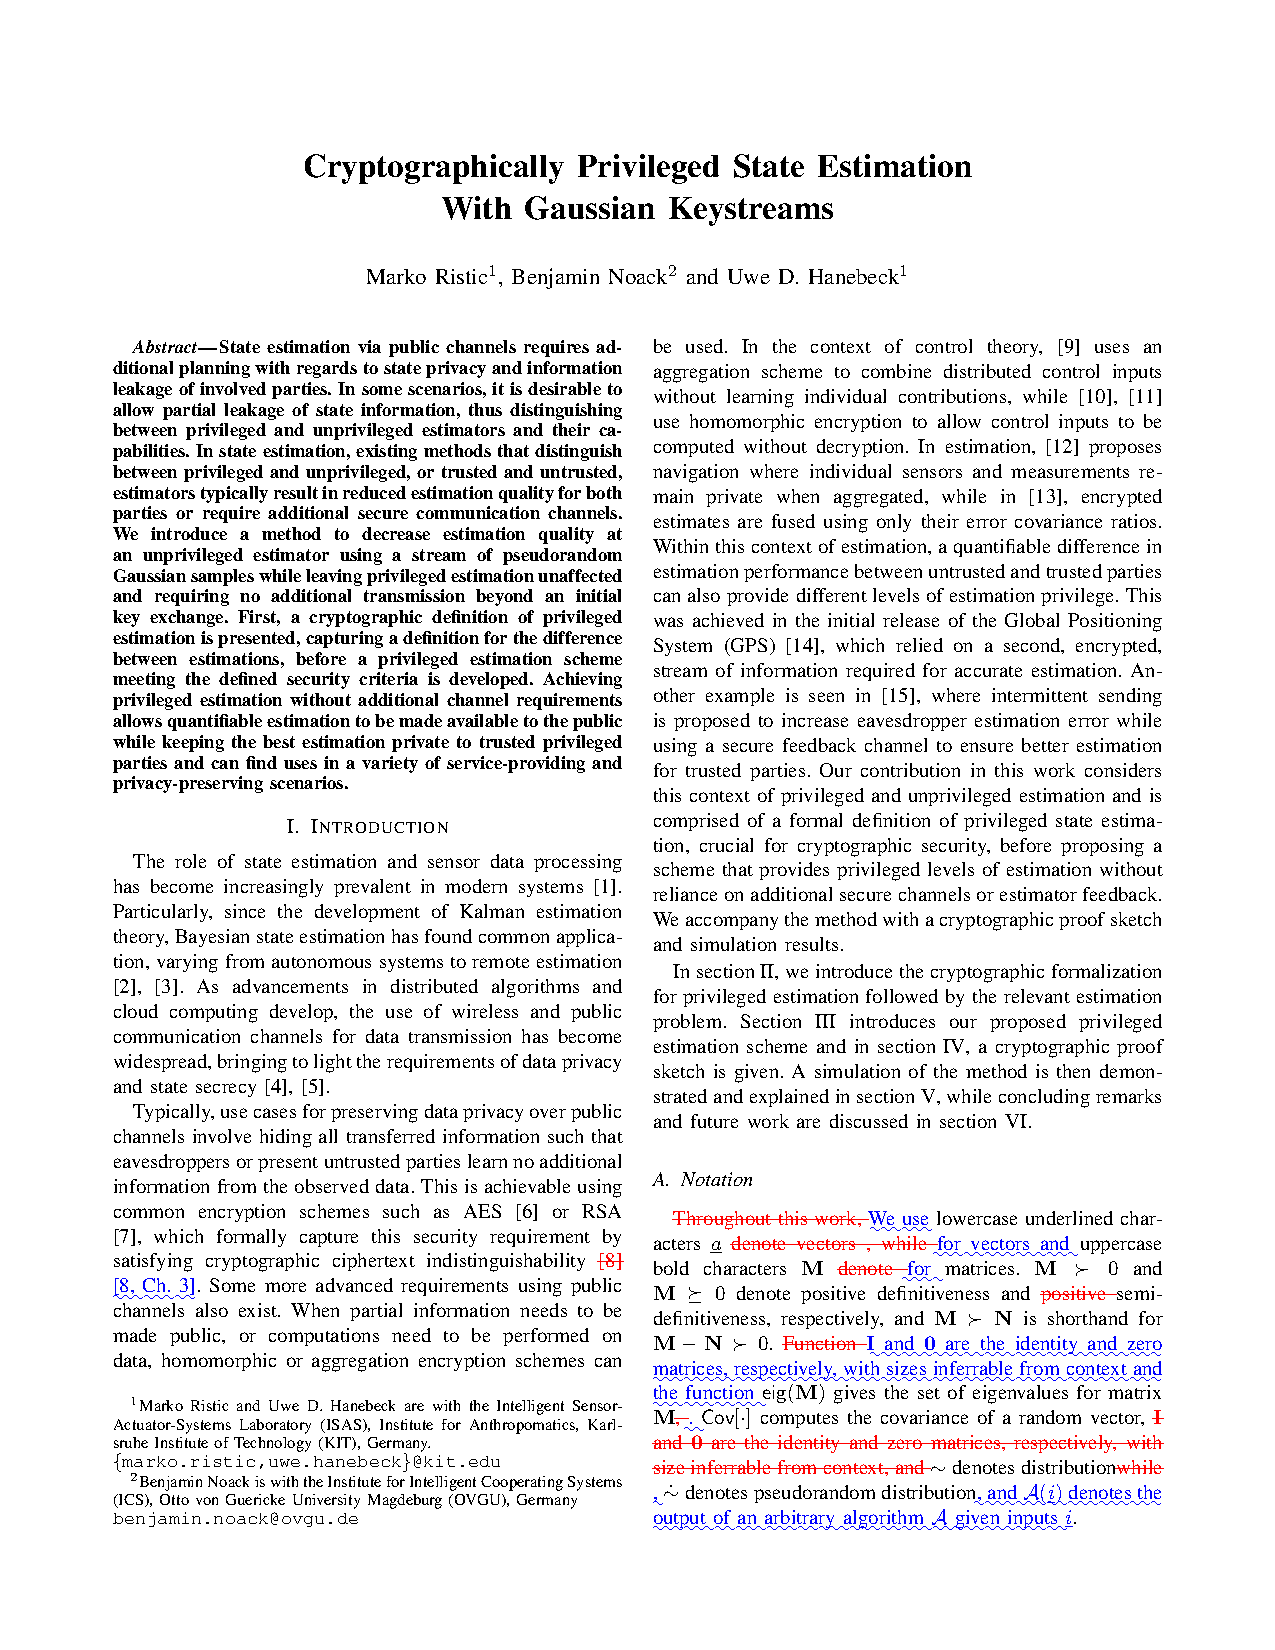
\includepdf[pages=-]{diff}

\end{document}